\section{Selecting the primitive for Efficient Architecture}

In designing our training methodology, \method, we aim to satisfy the following main requirements in the purview of embedded systems:

\begin{itemize}
\item {\em Privacy-}
The model should preserve the privacy of an individual's data record in the training set of the model against inference attacks.

\item {\em Accuracy-}
The drop in accuracy of the private model should be minimum as compared to the original accuracy.

\item {\em Efficiency-}
The private model should demonstrate high efficiency, i.e, energy, memory and computation efficiency.
\end{itemize}

To this end, we present \method --- a technique to construct deep neural network algorithms that are optimized for efficiency and accuracy while ensuring privacy of the input data.
With \method, we present a novel approach of building NN models that with efficiency as a key property.
We argue that fixing a neural network architecture and then modifying the training algorithm to ensure privacy does not provide optimal balance between efficiency and accuracy.
On the contrary, our approach advocates building neural network architecture considering the strengths and drawbacks of the underlying algorithms to design efficient neural networks.
We assert that this is a practical solution as deep learning algorithms are flexible with respect to their architectures i.e., different neural network models can be trained to achieve the same accuracy for a given dataset.



\subsection{Efficiency Optimization Algorithms}

In designing \method, we make several design choices with the goal of achieving efficiency over existing solutions.
The most important among them is the selection of the underlying algorithm to design Neural Networks with high efficiency.
Several state of the algorithms are currently adopted such as, however, these algorithm do not provide the required efficiency guarantees equally and the different algorithms enhances different aspects of efficiency.
These differences makes it difficult to decide which primitive is the best fit for designing a privacy-preserving system for a particular application.
Therefore, we first outline the desirable properties specifically for private neural network inference and then compare these algorithms with respect to these properties (as shown in Table~\ref{tbl:comparison}).
We select an efficient design scheme for neural networks that satisfies all our requirements.

We specifically select the three state of the art techniques:
\begin{itemize}
\item Model Compression through pruning redundant parameters and nodes
\item Quantization to lower the precision of model parameters and activations
\item Off-the-shelf neural network architectures specifically designed for efficiency
\end{itemize}

\noindent\textbf{Model Compression (Pruning).}

Network Pruning: Neural Networks are generally overparameterised. Hence, a large amount of weights are redundant adn can be removed (set to zero) referred to as pruning.
Aggressive pruning, however, requires to finetune the model to ensure no loss in the accuracy. Typically, this is done by removing the least significant nodes in the network by computing a threshold using the senstitivity hyperparameter which is used to estimate the percentile of values.

\[
    f(W)=
\begin{cases}
    0, & \text{if } w\geq T\\
    0, & \text{if } w\leq -T\\
    w,  & \text{otherwise}
\end{cases}
\]

The original pruning requires the model to be retrained after pruning to restore accruacy while ensuring lower network size.
Further, computation on these sparse parameter matrices using specialized accelerators enable to avoid computation on 0's lower the computation complexity significantly and increasing the overall inference speed.
Prior work has indicated that over 80\% of the parameters can be pruned and the accuracy can be restored after retraining.

Sparsity: Sparsity reduces some of the values in the network close to zero replaces them as zero. This results in the distribution with two modes instead of a single gaussian distribution for the parameters.
The sparsity constraint ensures that the parameters in the middle are zeroed out while the parameter values near the tail end are updated.

Sparse weights can be stored in a compressed format in the hardware using the compressed sparse row or column format which reduces the overall memory bandwidth[].
The decision on whether the computation is done is based on the parameter value which requires additional logic, i.e, replace output as zero without computation if parameter value is zero else perform the computation.
This also benefits in usage with SIMD or data parallel architectures and improves compression and reduces overall storage cost by using indices of weights with a zero values instead of actually storing zero values in the memory for each occurance.


\noindent\textbf{Quantization.} Quantization reduces the precision of the operands while techniques such as pruning, sparsity reduce the number of model operation and model size.
Quantization maps parameters/activtions to a smaller set of quantization levels [qunaitized neural networks].
The ultimate goal is to minimize the error between the reconstructed data from hte quantized levels and the original data.
The number of quantized levels reflects the precision and ultimately the nuber of bits required to represent the data (log2(number of levels))
Reducing precision results in lower number of bits to represent the data which results in a lower storage cost (parameters) and/or computation cost (activation). less are and less energy [M Horowitz]
For instance, using kbits instead of 32 bits or 64 bits weights reduces the storage cost by 32/k or 64/k and hence, requires lower number of parameters to be read form the memory which further improves the energy efficiency by 32/kx or 64/kx.

The precision can be reduced aggresively to a single bit to get binary nets. Here, the weights  and activation are binarized during inference to take values \{-1,+1\} [binaryconnect, binarynet]. This allows to reduce the MAC operation to an XNOR however, with a singificant accuracy loss[xnor-net].
Several optimisaition have been considered to reduce the loss such as multiplying the outputs with a scaling factor to recover the dynamic range( weights become -w and w), keeping the first and last layer as 32 bit floating point precision and performing normatlisation before convolution to reduce the dynamic range of activations.
Further, hybrid and varying bit precision of weights and activations have been used in Dorefanet, HWGQnet and QNNs to reduce the qunatization loss.
Further, there are benefits for allowing weights to be zero (-w, 0, w) although this requires an additional bit per weight compared to binary weights, the sparsity can be used to reduce computation and storage cost [Ternary weight networks, trained ternary quantization].
Here, we consider two cases: uniform quanrization
Weight sharing forces several weight values to share a single value which reduces the number of unique weights in the model.
The weights are grouped using hashing function or k means algorithm and one value is assigned to each group.
A codebook is then built to map each grou of weights to its shared value. accordingly, the index to the corresponging group in the codebook is strored for each position n the filter rather than a eright value. This leads to a two step process to fetch the weights:
(a) read the group index from the weight memory and (b) using the griup index read the value of weight from the codebook or dictionary.

In this work, we specifcally consider the case of aggreesive quantization where the parameters and activations are binarized.

YODANN

\noindent\textbf{Off-the-Shelf Efficient Architectures.}

Morphnet, Mobilenet squeezenet, netadapt

MobileNet~\cite{conf/cvpr/SandlerHZZC18}
SqueezeNet~\cite{DBLP:journals/corr/IandolaMAHDK16}
morphnet~\cite{46505}
netadapt~\cite{eccv_2018_yang_netadapt} automatically adapts a pre-trained deep neural netwo incorporates direct metrics into its adaptation algorithm
Compact Network Architectures: The number of parameters and complexity of etwork can be optimized by careful design of the network architecture itself.
Here, instead of replacing larger filters with a set of smaller filters which have fewer weights in total when the filters are applied sequentially they have same overall receptive field.
For instance, one 5x5 filter can be replace with 2 3x3 filters. 1x1 convolutional layers can be used to reduce the number of channels in output feature map and hence the overall computation.
Forexample,32 ltersof1x1x64can transform an input with 64 channels to an output of 32 channels and reduce the number of  lter channels in the next layer to 32. SqueezeNet uses many 1 x 1  lters to aggressively reduce the number of weights [157]. It proposes a  re module that  rst “squeezes” the net- work with 1 x 1 convolution  lters and then expands it with multiple 1 x 1 and 3 x 3 convolution  lters.
It achieves an overall 50x reduction in the number of weights compared to AlexNet, while maintaining the same accuracy
Replace 3x3 filters with 1x1 filters.Given a budget of a certain number of convolutionfilters,  we will choose to ma
ecrease the number of input channels to 3x3 filters.Consider a convolution layerthat is comprised entirely of 3x3 filters. , to maintain a small total number of parametersin a CNN, it is important not only to decrease the number of 3x3 filters (see Strategy 1 above), butalso to decrease the number ofinput channelsto the 3x3 filters.  We decrease the number of inputchannels to 3x3 filters usingsqueeze layers, which we describe in the next section.
Downsample late in the network so that convolution layers have large activationmaps.In a convolutional network, each convolution layer produces an output activation map witha spatial resolution that is at least 1x1 and often much larger than 1x1.


\subsection{Comparing Efficiency and Privacy}

\begin{table}[!htb]
\begin{center}
\renewcommand\arraystretch{1.5}
\fontsize{6.7pt}{6.7pt}\selectfont
\begin{tabular}{|l|l|l|l|}
\hline
 & Compression & Quantization & Architecture  \\
\hline
Computation & $\smark$  & $\cmark$   & $\xmark$ \\
\hline
Memory &  $\smark$ & $\cmark$   & $\cmark$ \\
\hline
Energy &  $\cmark$   & $\cmark$   & $\xmark$ \\
\hline
Privacy &  $\xmark$   & $\cmark$   & $\smark$ \\
\hline
\end{tabular}
\end{center}
\caption{$\checkmark$$\times$ indicates additional hardware optimization required in order to achieve efficiency.Comparison of different algorithms for efficient Deep learning.}
\label{tbl:comparison}
\end{table}


In comparing the three algorithms on the basis of efficiency, we define three aspects of efficiency, namely, computation efficiency, memory efficiency and energy efficiency.

\noindent\textbf{Computation Efficiency.} In order to measure the number of operations performed in a cycle, we first define the aspect of computation efficiency.
A model with computation efficiency has lower number of operations compared to the non-efficient counter part for the same architecture.
This number of operations, referred to as FLOPS, is directly correlated to the Mulitply-Accumulate (MAC) operations in the forward pass which includes the matrix-vector multiplications between the parameters of a layer and input activations from pervious layer.
Design of efficient Neural Network architectures replaces the complex matrix-vector multiplications by multiple matrix-vector multiplications with smaller dimensions.
This reduces the overall number of parameters but it has been shown empirically\footnote{https://github.com/albanie/convnet-burden} that this does not necessarily reduce the number of multiply accumulate operations or FLOPS [ANANALYSIS  OFDEEPNEURALNETWORKMODELSFORPRACTICALAPPLICATIONS].
For models with binarized parameters and activations the MAC operations can be replaced by binary operations such as XNOR and the maxpool operations can be replaced by OR operation, while the activations can be replaced by checking the parity bit (denotes the sign) operation and hence reducing the FLOPS drastically[XONN].
In case of parameter pruning, achieving efficiency requires additional hardware optimization. Particularly, instead of actually computing the the multiplications with "0"pruned values, the hardware optimization enable the user to skip the computation and replace the output by a "0" directly.
run faster with smaller bit width and higher throughput

energy benfit by reducing the memory access to the Hardware

\noindent\textbf{Memory Efficiency.} The total memory required by the model which includes the number of parameters $\times$ precision of each parameter gives the estimate of the static memory storage required.
However, the memory intitialization during inference computation requires additional memory storage to store the intermediate computation which have been found to be correlated to the size of the static memory storage of the model [ANANALYSIS  OFDEEPNEURALNETWORKMODELSFORPRACTICALAPPLICATIONS].
Off the shelf models are designed to specifically reduce the memory footprint. For examples, the memory footprint of Squeezenet and MobileNet is 5MB and 14Mb compared to 250Mb of Alexnet and >500Mb of VGG architectures.
Lowering the precision of the model from 64/32 bit  floating point to binary precision results in a direct reduction of 64x or 32x in the overall memory footprint of the model.
However, in case of model compression the model parameters which are pruned are simply replaced by a "0" value. Hence, storing even the "0" parameter takes up memory and does not necessarily decrease the overall memory footprint.
The benefits of model compression can be exploited to reduce the memory only when the hardware optimizations are employed by storing all the zero parameters and exploit the sparsity to only have an additional codebook to indicate the indices with zeroed parameters.

exploit sparsity by skipping memory access an computation; requires additional hardware to check for "0" pruned values.
pruning optimal brain damage: requires retraining

\noindent\textbf{Energy Efficiency.} We measure the energy consumpotion in terms of Inference/J or Inference/S/W Cost inference/s/\$.
This is particularly important as it relates to the cost incurred for running the embedded device for longer duration where each kJ is mapped to cost in money.
As noted in [][], desining efficient Neural Networks does not necessarily result in lowering the energy consumption.
Hence, efficient architectures do not lower the overall energy consumption.
On the other hand, quantization drastically reduces the energy consumption compared to full precision models.
Particularly, a model with 64bit or 32 bit floating point precision when quantized to binary precision, the resultant reduction in energy concumption decreases drastically.
Within a fixed number of cycles, low precision models can move larger number of parameters fetched compared to full precision model.
The total energy consumption of off the shelf architecture are close to the other state of the art architectures and lowering the memory footprint by a careful choice of Hyperparameters does not necessarily result in higher energy efficiency.

number of weights is not a good metrics for energy. important to take in account the data types, memory access .. and not easy to find energy consumption.
Energy evaluation methodology per layer and per memory hierarchy CVPR 2017 yang et al.
Squeezenet does not necessarily consume less energy than alexnet ..Pruning does reduce the energy but smaller improvement.

For every MAC, we have t access three information memory read: filter weight, image pixel and partial sum from previous layer and one write to store the computed output.
The access to the memory is around 2x higher energy consumption compared to the actual MAC operation and hence, memory access is the bottleneck.
additional hardware optimization optimized the dataflow processing with reuse of weights, outputs as part of spatial architecture to improve performance.

throughput and energy gains requires hardware optimization. reduce size of operands for storage and compute
reduce the number of operations by designing compact models, pruning and exploiting sparsity (special hardware required).

Comparison of efficiency have been widely studied for all the three cases and we refer to [][][] for more details about the computation, energy and memroy efficiency of such optimization techniques.

\noindent\textbf{Privacy Leakage.}

However, so far the privacy implication of optimization of deep neural networks have bot been studied.
To this extent, we address this gap and compare different optimizations based on the privacy leakage.

\begin{table}[!htb]
\begin{center}
\renewcommand\arraystretch{1.5}
\fontsize{6.7pt}{6.7pt}\selectfont
\begin{tabular}{|c|c|c|c|c|c|}
\hline
\textbf{Architecture} & \textbf{Train}  & \textbf{Test}  & \textbf{Inference}  & \textbf{Parameters} & \textbf{Memory} \\
 & \textbf{Accuracy} & \textbf{Accuracy} & \textbf{Accuracy} & & \textbf{Footprint} \\
\hline
SqueezeNet & 88.21\% & 81.92\% & \cellcolor{green!25}53.07\% & 1.2M & 5 MB\\
MobileNetV2 & 97.50\% & 87.24\% & \cellcolor{green!25}55.57\% & 3.5M & 14 MB\\
\hline
AlexNet & 97.86\% & 80.34\% & \cellcolor{red!25}60.40\% & 61M & 240 MB\\
VGG11 & 99.13\% & 86.43\% & \cellcolor{red!25}58.04\% & 132M & 507 MB\\
VGG16 & 99.58\% & 88.95\% & \cellcolor{red!25}58.70\% & 138M &  528 MB\\
VGG19 & 99.09\% & 88.18\% & \cellcolor{red!25}57.85\% & 143M & 549 MB\\
\hline
\end{tabular}
\end{center}
\caption{Model complexity influences the membership inference leakage. Model specifically designed for efficiency leak less information.}
\label{stdarch}
\end{table}

\begin{figure}[hb!]
\resizebox{0.8\columnwidth}{!}{%
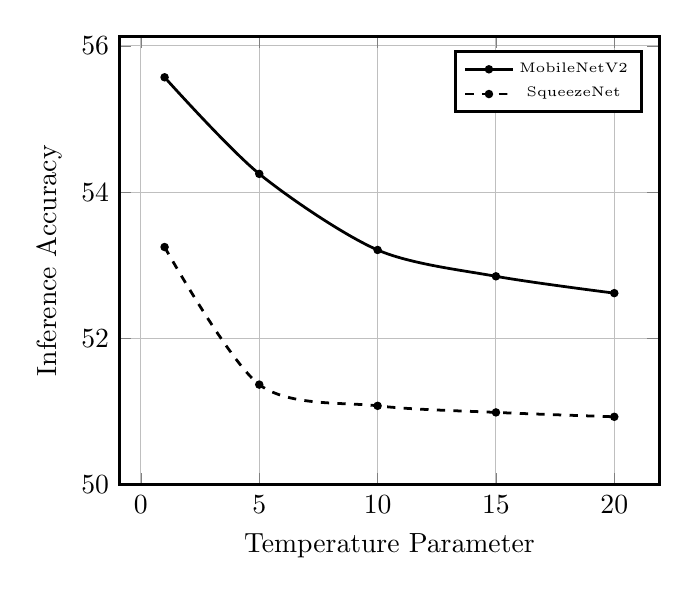
\begin{tikzpicture}
\begin{axis}[
legend style={font=\tiny},
legend pos =  north east,
line width=1.0pt,
mark size=1.0pt,
ymin=50,
legend entries={MobileNetV2, SqueezeNet},
ylabel={Inference Accuracy},
xlabel={Temperature Parameter},
% extra x ticks={1,10,...,400},
% extra y ticks={0,0.5,...,10},
% extra y tick labels={},
% extra x tick labels={},
% extra x tick style={grid=major},
% extra y tick style={grid=major},
grid=major
]
\addplot[
    color=black,
    solid,
    mark=*,
    mark options={solid},
    smooth
    ]
    coordinates {
    (1,55.57)(5,54.25)(10,53.21)(15,52.85)(20,52.62)
      };
\addplot[
      color=black,
      dashed,
      mark=*,
      mark options={solid},
      smooth
    ]
    coordinates {
    (1,53.25)(5,51.37)(10,51.08)(15,50.99)(20,50.93)
      };
\end{axis}
\end{tikzpicture}
}
\caption{The privacy leakage of models designed for efficiency (SqueezeNet and MobileNet) can be reduced by increasing the softmax temperature. }
\end{figure}






WHy pruning/ model compression is not the best choice.. leaks more information

\begin{figure*}[ht!]
\begin{center}% note that \centering uses less vspace...
\resizebox{2\columnwidth}{!}{%
\begin{tabular}{lllll}


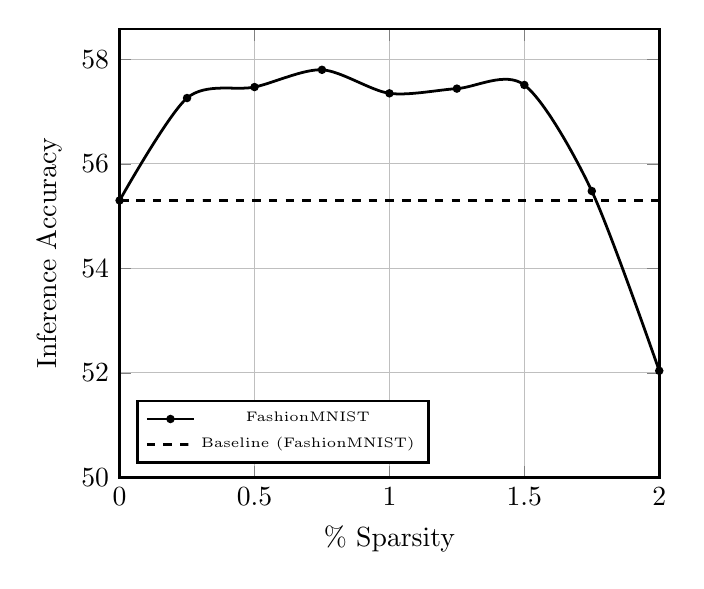
\begin{tikzpicture}
\begin{axis}[
legend style={font=\tiny},
legend pos =  south west,
line width=1.0pt,
mark size=1.0pt,
ymin=50,
xmin=0,
xmax=2,
legend entries={FashionMNIST, Baseline (FashionMNIST)},
ylabel={Inference Accuracy},
xlabel={\% Sparsity},
% extra x ticks={1,10,...,400},
% extra y ticks={0,0.5,...,10},
% extra y tick labels={},
% extra x tick labels={},
% extra x tick style={grid=major},
% extra y tick style={grid=major},
grid=major
]
\addplot[
    color=black,
    solid,
    mark=*,
    mark options={solid},
    smooth
    ]
    coordinates {
    (0,55.30)(0.25,57.26)(0.5,57.47)(0.75,57.80)(1,57.35)(1.25,57.44)(1.5,57.51)(1.75,55.48)(2,52.04)
      };
\addplot[
    color=black,
    dashed,
    smooth
    ]
    coordinates {
    (0,55.30)(0.25,55.30)(0.5,55.30)(0.75,55.30)(1,55.30)(1.25,55.30)(1.5,55.30)(1.75,55.30)(2,55.30)
      };
\end{axis}
\end{tikzpicture} &


%
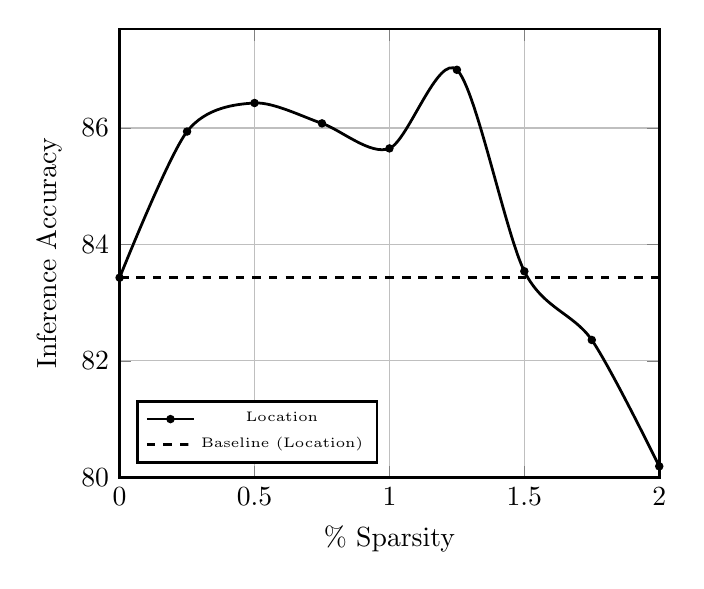
\begin{tikzpicture}
\begin{axis}[
legend style={font=\tiny},
legend pos =  south west,
line width=1.0pt,
mark size=1.0pt,
ymin=80,
xmin=0,
xmax=2,
legend entries={Location, Baseline (Location)},
ylabel={Inference Accuracy},
xlabel={\% Sparsity},
grid=major
]
\addplot[
    color=black,
    solid,
    mark=*,
    mark options={solid},
    smooth
    ]
    coordinates {
    (0,83.43)(0.25,85.94)(0.5,86.43)(0.75,86.08)(1,85.65)(1.25,87.00)(1.5,83.54)(1.75,82.36)(2,80.19)
      };
\addplot[
    color=black,
    dashed,
    smooth
    ]
    coordinates {
    (0,83.43)(0.25,83.43)(0.5,83.43)(0.75,83.43)(1,83.43)(1.25,83.43)(1.5,83.43)(1.75,83.43)(2,83.43)
      };

\end{axis}
\end{tikzpicture} &





%
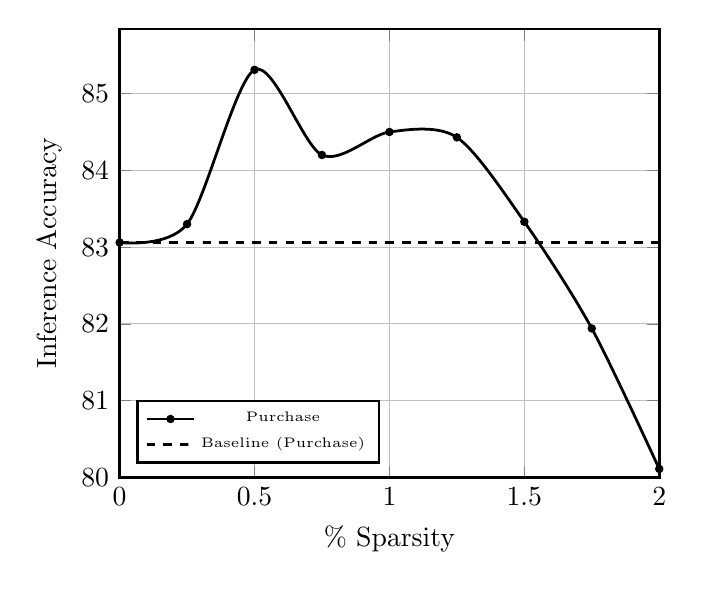
\begin{tikzpicture}
\begin{axis}[
legend style={font=\tiny},
legend pos =  south west,
line width=1.0pt,
mark size=1.0pt,
ymin=80,
xmin=0,
xmax=2,
legend entries={Purchase, Baseline (Purchase)},
ylabel={Inference Accuracy},
xlabel={\% Sparsity},
grid=major
]
\addplot[
    color=black,
    solid,
    mark=*,
    mark options={solid},
    smooth
    ]
    coordinates {
    (0,83.06)(0.25,83.30)(0.5,85.31)(0.75,84.20)(1,84.50)(1.25,84.43)(1.5,83.33)(1.75,81.94)(2,80.11)
      };
\addplot[
    color=black,
    dashed,
    smooth
    ]
    coordinates {
    (0,83.06)(0.25,83.06)(0.5,83.06)(0.75,83.06)(1,83.06)(1.25,83.06)(1.5,83.06)(1.75,83.06)(2,83.06)
      };

\end{axis}
\end{tikzpicture}


\end{tabular}
}
\caption{.}
\label{fig:loss}
\end{center}
\end{figure*}

\begin{figure*}[ht!]
\begin{center}% note that \centering uses less vspace...
\resizebox{2\columnwidth}{!}{%
\begin{tabular}{lllll}


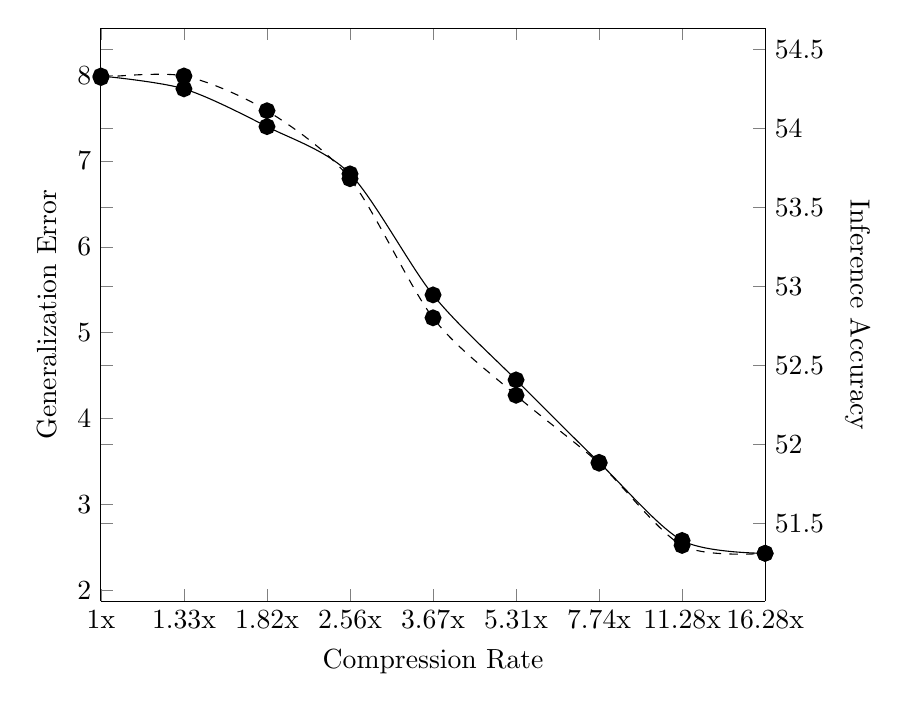
\begin{tikzpicture}
% let both axes use the same layers
\pgfplotsset{set layers}
%
\begin{axis}[
scale only axis,
line width=2.0pt,
mark size=2.0pt,
xmin=0,xmax=8,
ylabel={Generalization Error},
axis y line*=left,
xlabel={Compression Rate},
xtick={0,1,2,3,4,5,6,7,8},
xticklabels={1x, 1.33x, 1.82x, 2.56x, 3.67x, 5.31x, 7.74x, 11.28x, 16.28x}
]
\addplot[
    color=black,
    solid,
    mark=*,
    mark options={solid},
    smooth
    ]
    coordinates {
    (0,7.99)(1,7.84)(2,7.4)(3,6.85)(4,5.44)(5,4.45)(6,3.49)(7,2.58)(8,2.43)
      };
\end{axis}

\begin{axis}[
scale only axis,
line width=2.0pt,
mark size=2.0pt,
xmin=0,xmax=8,
ylabel near ticks, yticklabel pos=right,
ylabel={Inference Accuracy},
ylabel style = {rotate=180},
axis x line=none
]
\addplot[
    color=black,
    dashed,
    mark=*,
    mark options={solid},
    smooth
    ]
    coordinates {
    (0,54.32)(1,54.33)(2,54.11)(3,53.68)(4,52.80)(5,52.31)(6,51.88)(7,51.36)(8,51.31)
        };
\end{axis}
\end{tikzpicture} &

%
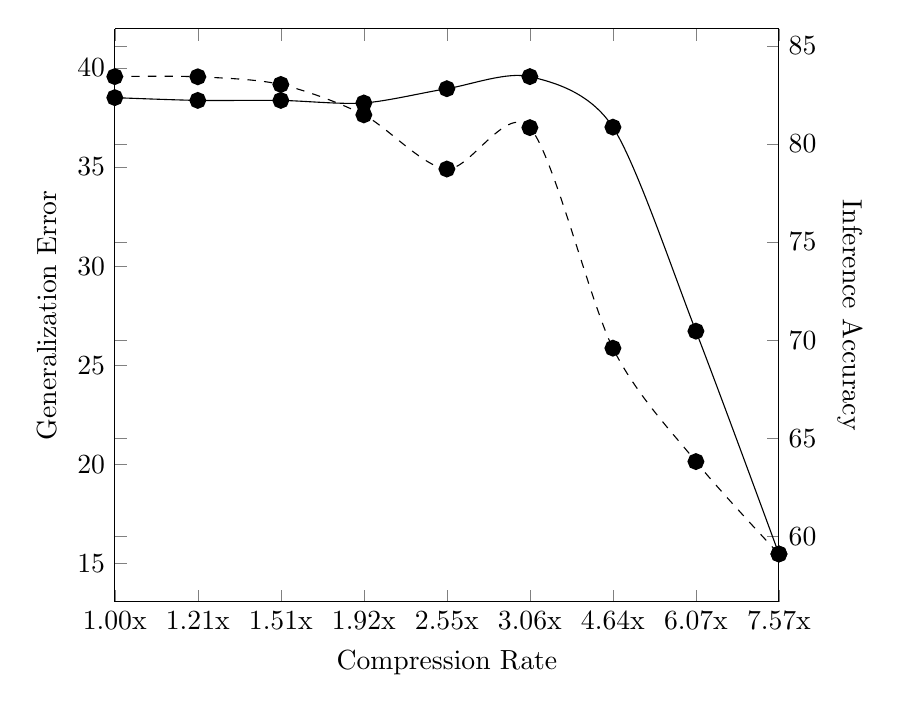
\begin{tikzpicture}
% let both axes use the same layers
\pgfplotsset{set layers}
%
\begin{axis}[
scale only axis,
line width=2.0pt,
mark size=2.0pt,
xmin=0,xmax=8,
ylabel={Generalization Error},
axis y line*=left,
xlabel={Compression Rate},
xtick={0,1,2,3,4,5,6,7,8},
xticklabels={1.00x, 1.21x, 1.51x, 1.92x, 2.55x, 3.06x, 4.64x, 6.07x, 7.57x}
]
\addplot[
    color=black,
    solid,
    mark=*,
    mark options={solid},
    smooth
    ]
    coordinates {
    (0,38.5)(1,38.36)(2,38.36)(3,38.23)(4,38.95)(5,39.56)(6,37.01)(7,26.72)(8,15.48)
      };
\end{axis}

\begin{axis}[
scale only axis,
line width=2.0pt,
mark size=2.0pt,
xmin=0,xmax=8,
ylabel near ticks, yticklabel pos=right,
ylabel={Inference Accuracy},
ylabel style = {rotate=180},
axis x line=none
]
\addplot[
    color=black,
    dashed,
    mark=*,
    mark options={solid},
    smooth
    ]
    coordinates {
    (0,83.43)(1,83.42)(2,83.03)(3,81.48)(4,78.72)(5,80.83)(6,69.59)(7,63.81)(8,59.10)
        };
\end{axis}
\end{tikzpicture} &





%
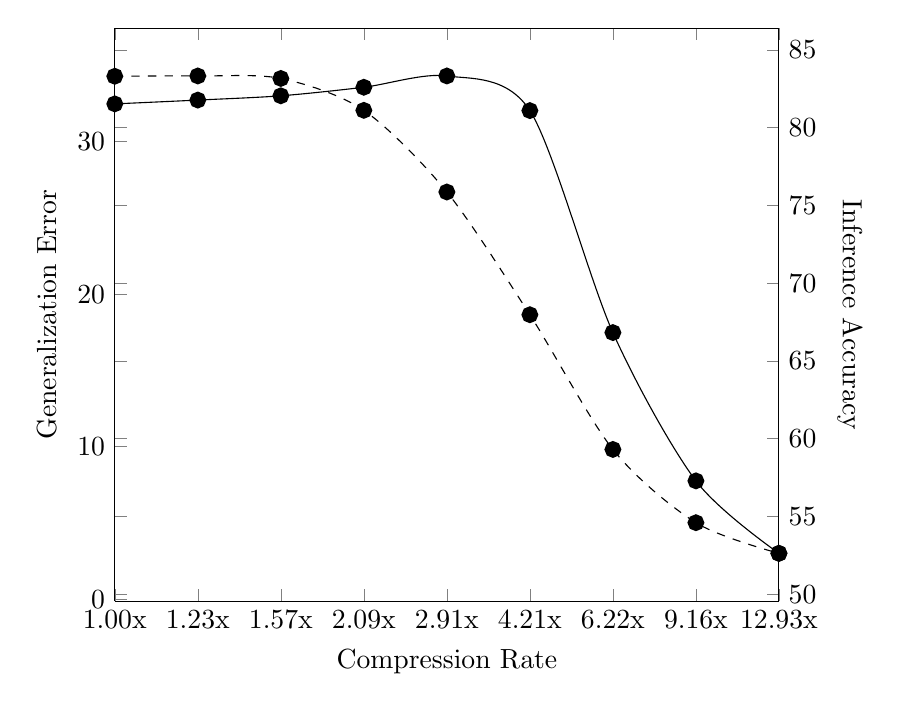
\begin{tikzpicture}
% let both axes use the same layers
\pgfplotsset{set layers}
%
\begin{axis}[
scale only axis,
line width=2.0pt,
mark size=2.0pt,
xmin=0,xmax=8,
ylabel={Generalization Error},
axis y line*=left,
xlabel={Compression Rate},
xtick={0,1,2,3,4,5,6,7,8},
xticklabels={1.00x, 1.23x, 1.57x, 2.09x, 2.91x, 4.21x, 6.22x, 9.16x, 12.93x}
]
\addplot[
    color=black,
    solid,
    mark=*,
    mark options={solid},
    smooth
    ]
    coordinates {
    (0,32.47)(1,32.72)(2,33)(3,33.56)(4,34.3)(5,32.03)(6,17.48)(7,7.76)(8,3.01)
      };
\end{axis}

\begin{axis}[
scale only axis,
line width=2.0pt,
mark size=2.0pt,
xmin=0,xmax=8,
ylabel near ticks, yticklabel pos=right,
ylabel={Inference Accuracy},
ylabel style = {rotate=180},
axis x line=none
]
\addplot[
    color=black,
    dashed,
    mark=*,
    mark options={solid},
    smooth
    ]
    coordinates {
    (0,83.30)(1,83.32)(2,83.16)(3,81.11)(4,75.86)(5,67.97)(6,59.31)(7,54.60)(8,52.63)
        };
\end{axis}
\end{tikzpicture}


\end{tabular}
}
\caption{FashionMNIST(left) Purchase100(Center) Location(Right). Dashed is Inference accuracy, solid is generalisaton error}
\label{fig:loss}
\end{center}
\end{figure*}


\cite{45932}\cite{cap}
The capacity is measured using the mutual information, defined as a measure of the amount of information that one random variable contains about another random variable. The mutual information of a trained network with N input samples is calculated as follows:
\begin{equation}
I ( Y ; Y_{\theta}' | X ) = H ( Y | X ) - H ( Y | Y_{\theta}' , X )
\end{equation}
\begin{equation}
=N (1-(plog2 p+(1-p)log2 (1-p)) )
\end{equation}
where p is the mean classification accuracy for all samples under trained parameter theta. If the training accuracy is 1, the model memorizes all random samples and the I (Y ; Y' |X ) becomes the number
of samples N . If the training accuracy is 0.5, I (Y ; Y' |X ) goes to theta.
The accuracy, p, may vary depending on the training method of the model. We find N and p that maximize the mutual information of the networks by iteratively training the models.
X = \{$X_1,...,X_N$\},Xi $\in$ $(0,1)^{|N|}$
Y = $\{Y_1,...,Y_N\}$,$Y_i$ $\in$ (0,1),
Y' = $\{Y_1', ..., Y_N'\}, Y_i$' = f($\theta, X_i$),
where $f(\theta,X_i)$ is the predict of a network when the input is $X_i$. Under our experimental setting, both X and Y have uniform random distribution. Note that X and Y are independent as well as $Y_i$ and $Y_j$ when i not= j. Therefore
$P (Y_i|X_i) = P (Y_i) = 1/2$, and $H(Y) = H(Y_1, ..., Y_N ) = N H(Y_1) = N$.

And we use the network’s average accuracy p as a probability of Yi = Y'i, so that

\[
    P(Yi|Y'i)=
\begin{cases}
    p, & \text{if } Yi =Y'i\\
    (1 - p),  & \text{otherwise}
\end{cases}
\]

Finally, the equation is derived as:
\begin{equation}
I(Y;Y'|X)= H ( Y | X ) - H ( Y | Y' , X )
\end{equation}
\begin{equation}
= H ( Y ) - H ( Y | Y' ) = N -   H ( Y i | Y' i )
\end{equation}
\begin{equation}
= N -   H ( Y i | Y' i )
\end{equation}
\begin{equation}
=N-N plog2 p+(1-p)log2 (1-p)
\end{equation}
This captures
the amount of information stored in the parameters about the mapping between X and Y. To get an estimate of bits per parameter, we divide by the number of parameters,


\begin{figure*}[ht!]
\begin{center}% note that \centering uses less vspace...
\resizebox{2\columnwidth}{!}{%
\begin{tabular}{lllll}


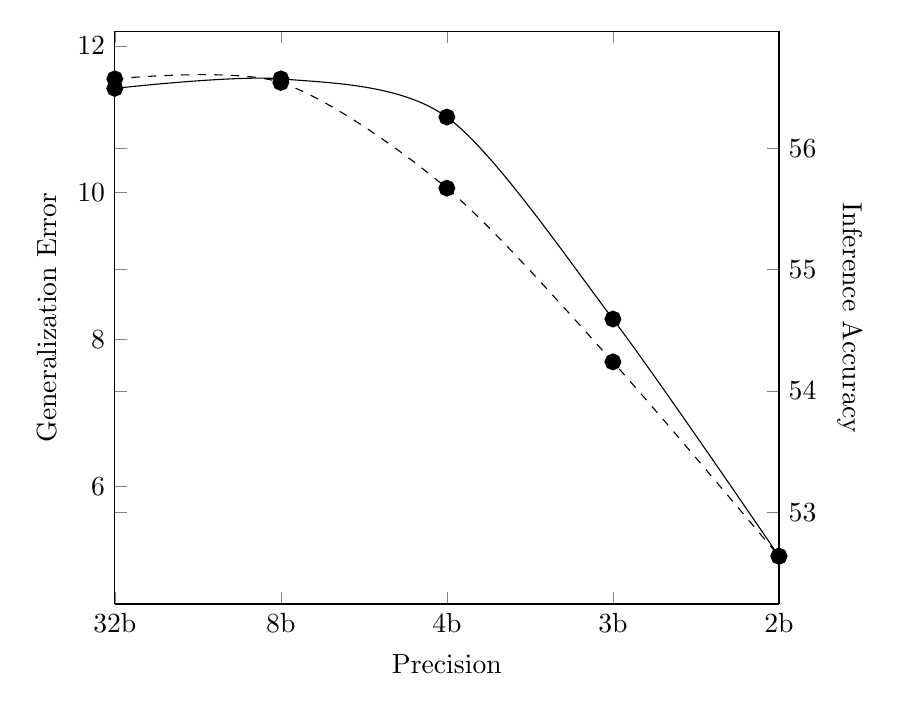
\begin{tikzpicture}
% let both axes use the same layers
\pgfplotsset{set layers}
%
\begin{axis}[
scale only axis,
line width=2.0pt,
mark size=2.0pt,
xmin=0,xmax=4,
ylabel={Generalization Error},
axis y line*=left,
xlabel={Precision},
xtick={0,1,2,3,4},
xticklabels={32b, 8b, 4b, 3b, 2b}
]
\addplot[
    color=black,
    solid,
    mark=*,
    mark options={solid},
    smooth
    ]
    coordinates {
    (0,11.42)(1,11.55)(2,11.03)(3,8.28)(4,5.05)
      };
\end{axis}

\begin{axis}[
scale only axis,
line width=2.0pt,
mark size=2.0pt,
xmin=0,xmax=4,
ylabel near ticks, yticklabel pos=right,
ylabel={Inference Accuracy},
ylabel style = {rotate=180},
axis x line=none
]
\addplot[
    color=black,
    dashed,
    mark=*,
    mark options={solid},
    smooth
    ]
    coordinates {
    (0,56.57)(1,56.54)(2,55.67)(3,54.24)(4,52.64)
        };
\end{axis}
\end{tikzpicture} &

%
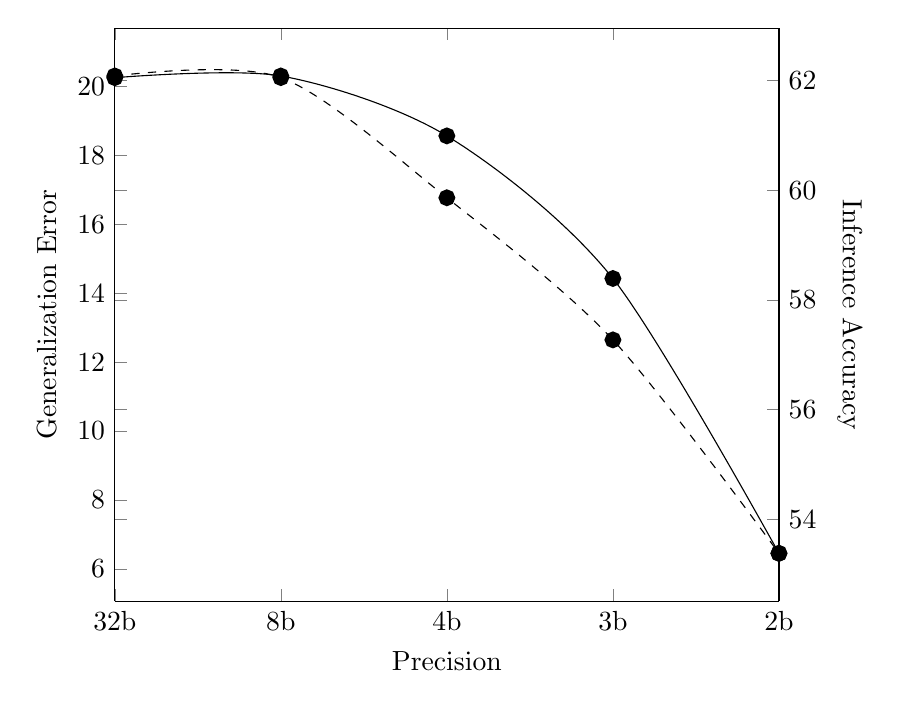
\begin{tikzpicture}
% let both axes use the same layers
\pgfplotsset{set layers}
%
\begin{axis}[
scale only axis,
line width=2.0pt,
mark size=2.0pt,
xmin=0,xmax=4,
ylabel={Generalization Error},
axis y line*=left,
xlabel={Precision},
xtick={0,1,2,3,4},
xticklabels={32b, 8b, 4b, 3b, 2b}
]
\addplot[
    color=black,
    solid,
    mark=*,
    mark options={solid},
    smooth
    ]
    coordinates {
    (0,20.26)(1,20.31)(2,18.57)(3,14.43)(4,6.45)
      };
\end{axis}

\begin{axis}[
scale only axis,
line width=2.0pt,
mark size=2.0pt,
xmin=0,xmax=4,
ylabel near ticks, yticklabel pos=right,
ylabel={Inference Accuracy},
ylabel style = {rotate=180},
axis x line=none
]
\addplot[
    color=black,
    dashed,
    mark=*,
    mark options={solid},
    smooth
    ]
    coordinates {
    (0,62.08)(1,62.05)(2,59.86)(3,57.27)(4,53.38)
        };
\end{axis}
\end{tikzpicture} &





%
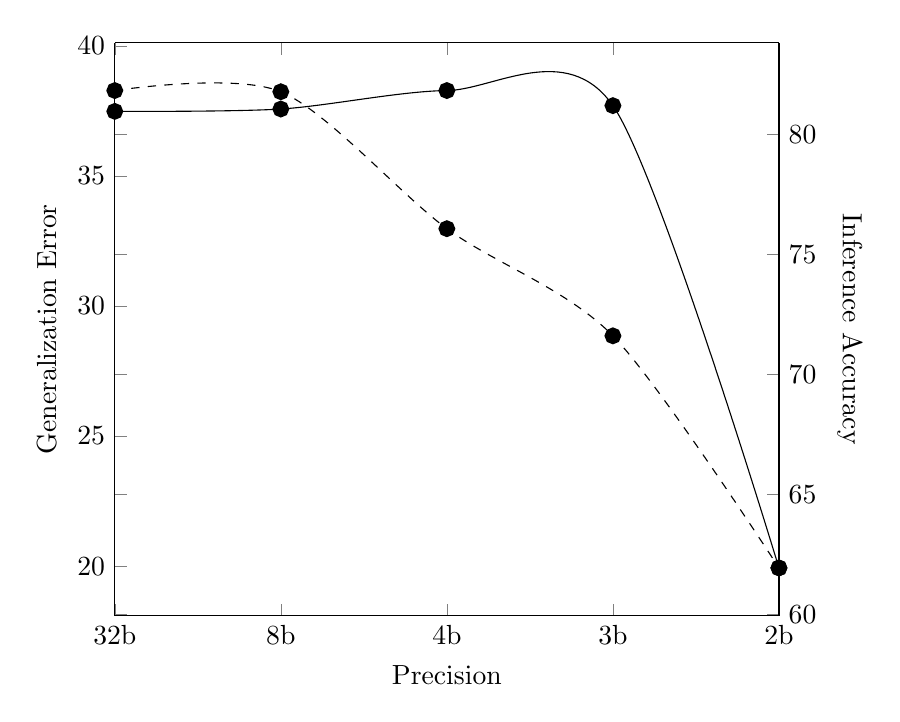
\begin{tikzpicture}
% let both axes use the same layers
\pgfplotsset{set layers}
%
\begin{axis}[
scale only axis,
line width=2.0pt,
mark size=2.0pt,
xmin=0,xmax=4,
ylabel={Generalization Error},
axis y line*=left,
xlabel={Precision},
xtick={0,1,2,3,4},
xticklabels={32b, 8b, 4b, 3b, 2b}
]
\addplot[
    color=black,
    solid,
    mark=*,
    mark options={solid},
    smooth
    ]
    coordinates {
    (0,37.48)(1,37.57)(2,38.28)(3,37.70)(4,19.93)
      };
\end{axis}

\begin{axis}[
scale only axis,
line width=2.0pt,
mark size=2.0pt,
xmin=0,xmax=4,
ylabel near ticks, yticklabel pos=right,
ylabel={Inference Accuracy},
ylabel style = {rotate=180},
axis x line=none
]
\addplot[
    color=black,
    dashed,
    mark=*,
    mark options={solid},
    smooth
    ]
    coordinates {
    (0,81.82)(1,81.77)(2,76.07)(3,71.61)(4,61.95)
        };
\end{axis}
\end{tikzpicture}


\end{tabular}
}
\caption{\underline{Pruning followed by Weight Sharing (Quantization).} While the retraining after pruning is necessary to restore the predictive accuracy, clustering the weights to reduce the precision lowers the inference accuracy (dashed line) risk while reducing the generalization error (solid line) for FashionMNIST(left), Purchase100(Center) and Location(Right) dataset.}
\label{fig:loss}
\end{center}
\end{figure*}

We evaluate the effectiveness of pruning followed by quantization which has been shown to have significant impact on reducing the model complexity through compression more significantly than either pruning or quantization alone.
We use the same model after pruning with Sensitivity since, it leaks the most information and evaluate the effective of quantization and whehter it can enable a good balance between test accuracy and inference accuracy.
